\documentclass[10pt,a4paper]{article}
\usepackage[utf8]{inputenc}
\usepackage{amsmath}
\usepackage{amsfonts}
\usepackage{amssymb}
\usepackage{graphicx}
\usepackage{cite}
\usepackage{ucs}
\usepackage{listings} %for code
\usepackage{color} %for code
\usepackage{ulem} %dobule underline
\usepackage[english]{babel}
\usepackage[margin=2.5cm]{geometry}
\usepackage[hidelinks]{hyperref}

\author{Stefan Klaus\\stk4@aber.ac.uk\\Aberystwyth, Wales}
\title{Major Project Documentation}

% defines how code will be shown
\definecolor{dkgreen}{rgb}{0,0.6,0}
\definecolor{gray}{rgb}{0.5,0.5,0.5}
\definecolor{mauve}{rgb}{0.58,0,0.82}
% still code
\lstset{frame=tb,
  language=Java,
  aboveskip=3mm,
  belowskip=3mm,
  showstringspaces=false,
  columns=flexible,
  basicstyle={\small\ttfamily},
  numbers=none,
  numberstyle=\tiny\color{gray},
  keywordstyle=\color{blue},
  commentstyle=\color{dkgreen},
  stringstyle=\color{mauve},
  breaklines=true,
  breakatwhitespace=true
  tabsize=3
}
\graphicspath{{./figures/}}
%%%%%%%%%%%%%%%%%%%%%%%%%%%%%%%%%%%%%
%	usefull stuff:
%	[3ex] is better than vspace{11pt}
%	\uuline{} gives a double underline
%	
%	\begin{figure}[h]
%	\includegraphics[width = 1\textwidth]{path_to_file}
%	\caption{caption_for_the_picture}
%	\label{Figure 1}
%	\end{figure}
%	
%	centering a small picture
%	\centerline{\includegraphics[width=0.9\textwidth]{file}}
%	
%	start code listing:
%	\begin{lstlisting}
%	\end{lstlisting}
%%%%%%%%%%%%%%%%%%%%%%%%%%%%%%%%%%%%
\begin{document}
\bibliographystyle{IEEEannot}
\maketitle
\newpage
\tableofcontents
\listoffigures
\newpage
\begin{flushleft}
\section{Background and Design}
\subsection{What the Project is about}
This project is about the map building using swarm intelligence.\\
The aspects of the project include SLAM(Simultaneous Localization And Mapping) as well as communication between a swarm of robots.\\
This document will disuse aspects such as robot localisation, deployment of the swarm, communication between robots and environment mapping.\\
My work is based on the research themes in these areas and I am using the robot simulator software Webots\textsuperscript{\texttrademark}. The mobile robot platform I am using is a virtual representation of the E-Puck robot. \\
The Programming will be done in C, using the Webots\textsuperscript{\texttrademark} API.\\[3ex]

One possible scenario for the program I am developing would be the mapping of an environment that would have become partially unknown after e.g. an nature catastrophe. I specify it this way since the team which would deploy this program on their robot swarm would most likely know the estimated size of the target environment, this is important in order to find an appropriate size for the robot swarm.\\
In such an scenario it is not always possible to achieve GPS coverage so the program should at its best function without the need for GPS localisation, so too find a localisation method which does not requires it is key. Another important features of the robot are obviously distance sensors, the E-Puck robot comes equipped with laser distance sensors, which I will use. Other features cover communication possibilities between robots, motor encoders which are needed for moving the robots in a controlled pattern and odometry calculations which will improve the movement and mapping significantly. \\[3ex]
While it is true that the E-puck robot platform is most likely not suitable for such a scenario I use it because of the time limitation for this project and its good integration inside the Webots\textsuperscript{\texttrademark} simulator. 


\subsection{Background}
\subsubsection{SLAM - Simultaneous Localization And Mapping}
The SLAM problem is a current research topic which is based on different localisation algorithms and using a range of different sensor to effectively map an target area. A lot of different approaches have been done and many research papers have been written, the one I am basing my project on being a paper about a SLAM solution designed for autonomous vehicles\cite{Dissanayake2001Solution}.\\
While the research area of this paper is based on a much larger scale and only using 1 vehicle in comparison to flock, it does still give me an insight upon the SLAM problem.\\
E.g. the problem with localisation in an dynamic environment, the paper tackles this problem by using global reference points and a millimetre wave radar, however for my project I do use an static environment and simple laser range finders. So this paper is only used a reference to the localisation problem, especially the idea of using "global" reference points for the created map.\\
As the test environment and the sensors available for the E-puck sensors are limited I will assume that the starting location of the robots is known.\\[3ex]

Another paper I read about this problem used an approach much more similar to my own project, by using different mobile robots which have no GPS access and simply use 2D laser range finders. However the approach described in this paper was based around the mapping of one "lead" robot and the traversing the same map again with a second robot using the map generated by the first for localisation purposes.\\
The second robot would then scan the target area again and refine the already generated map though using the (now stationary) first robot as an reference point. Since my project is planed about using multiple robot which scan the area at the same time it does still gives some information and idea about map sharing and improving. \\
Since my swarm will traverse the area at the same time it would be needed to share the map in real time and know the robot location in comparison to the first global referring point.  By implementing this I could rescan an area if a robot traverse an area another robot already scanned and refine the the final map by this. I will however look into real time sharing between different robots and can not say at this point if I will implement this in my final solution, it is however a interesting thought.\\[3ex]

\subsubsection{Deployment}
The deployment strategy is an important part of my project as it defines how effective the swarm will cover the target area which will define how long it will take to scan and map the whole area. Another important aspect is how many robots can the swarm hold and effectively deploy using the current deployment strategy. \\ 
One research paper I found proposed an solution of a communication network where the comm nodes keep track of the robots positions and guide them in directions which have not been explored in the last time period\cite{Batalin2003Coverage}. The paper uses a solution which is based on small comm nodes deployed by the robot, to make the solution fitting for my project I would have to define some of my E-pucks as communication nodes which remain on a fast position and guide the "scout" E-pucks based on area which have been least visited by the other robots.\\ 
This is certainly an possible solution however it could be considered a waste of robots in an small environment. Since I am using an simulator there is no communication range problem, but as my indentions are to make it as close to a possible real world application as possible I must still consider this.
That is why I am going to implement an maximum communication range for the robots however more about that can be found inside the "Communication" section. It is however an aspect to which I will come back later in my testing.\\[3ex]

Another paper proposed an solution which is based on an Nearest-Neighbour algorithm, meaning every robot must have always a minimum of "N" other robots inside its communication range\cite{Poduri2004Constrained}. In this solution to robots would emit signals to other robots which would manoeuvre the robots away from each other until only "N" robots remain inside the robots communication range. \\
This solution would cover a large area with the swarm fairly fast and also be adaptable for a swarm of any size, however a solution of moving the whole swarm in on direction would be needed in order to cover the whole target area, assuming the robot swarm is not big enough to cover it once completely deployed.
This would therefore need both a lead robot which decides the movement of the swarm and communication robots which would always have at least 1 link to another comm robot in order to have a communication line back to the lead robot. \\
This is one of two 2 deployment strategies I will try to implement during the testing period and try to find out which one would be more fitting for my project.\\[3ex]

\subsubsection{Communication}
While it is possible for me to transfer information easily between robots since I am using a simulator I am still trying implement it as close to a realistic scenario as possible, meaning that the communication range for the robots is limited. In an realistic scenario every robot would have to send the acquired map back to the static start point/lead robot so that an overall map of the environment can be created. \\
Since the communication range for such small robots is limited and can be even further obstructed through obstacles like walls it is important to designated some robots as communication nodes. Such comm nodes would than remain stationary and link the "scout" robots, which do the exploration, back to do the lead robot. \\
Obviously the most effective way to do this is by implementing different behaviour patterns for scouts or comm robots, and implement a decision model which allows the robot to change between either pattern as the needs of the swarm change. E.g. in the start of the exploration no comm robots will be needed as the robots would most likely be inside the comm range of the lead robot, though this may change if the swarm is big and spread out enough. \\[3ex]

To surpass the problems of obstacles obstructing the communication the comm robots would need to position them self on logical places i.e. in order to scan a room it would be important that a comm robot places it self inside, or close to, the doorway so that others can explore the room and still communicated back to the rest of the swarm. The robot would need to stay inside the doorway as signals can not always travel through walls and the energy reserves of mobile robots are limited so they most likely can not send high power signals. \\
I have yet to decide how I am going to implement the communication part of in the project as I am not sure if the E-puck models implemented inside the simulator are able to send signals to other robots. While I know that it is able to transfer signals through the E-puck's laser sensors I do not know if I will implement it as this is fairly difficult and time consuming. I will come back to this should I have enough time available at the end of the project or if no other alternative can be found.\\[3ex]

The theory of what I am going to implement uses a defined maximum communication range for the robots and a grouping strategy which specifies that each scout robot need to stay in contact which at least 1 comm robot while the comm robots always need at least 1 other comm robot inside their communication range. If implemented correctly the comm robots would on this way create a communication link back to the lead robot/starting location which the scout robots can use to transfer all new information back.\\

\begin{figure}[h]
\centering
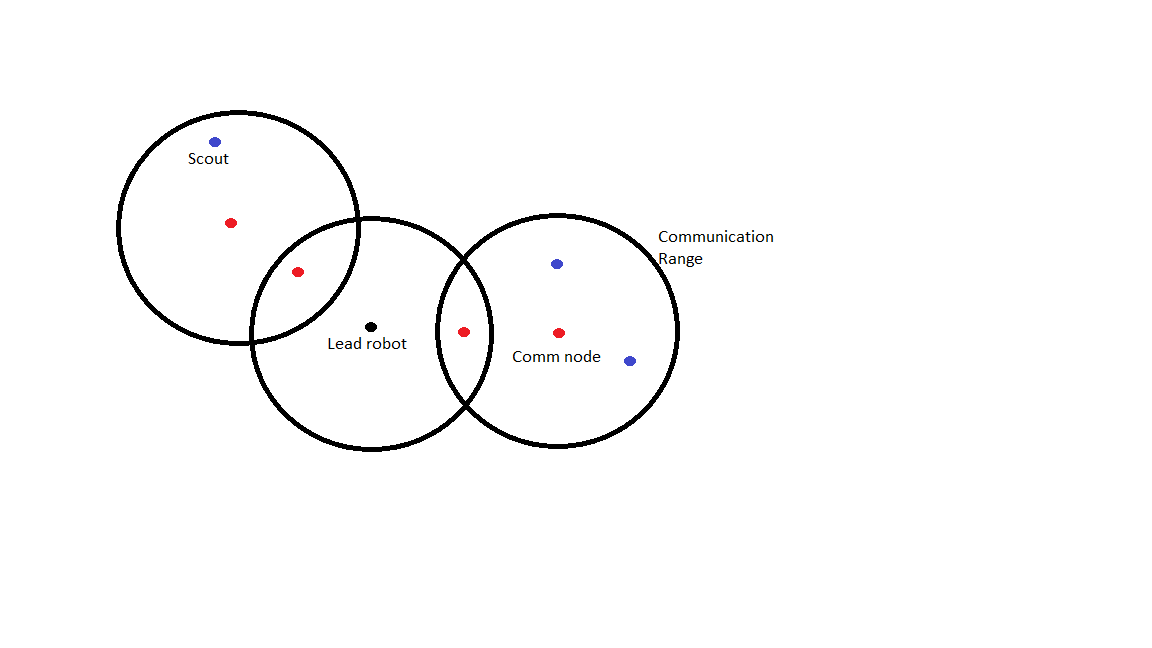
\includegraphics[width = 0.8\textwidth]{figures/comm_example.png} 
\caption{An example of the communication link}
\label{Picture 1}
\end{figure}

Figure 1 shows one possible example of the communication link, where the lead robot/ or in some cases a stationary uplink point is in the center and the communication robots(in red) placed in such positions that their comm range overlaps the comm range of other robots and the lead robot. \\
This configuration allows the scouts(in blue) to move and explore anything inside the communication range of the different comm robots. When the robots at the right side of the figure would now try to move outside the comm range one of them would have to change their behaviour pattern to "communication mode" at the outer range of the other comm nodes range while the last remaining scout continuous exploring in this direction. \\
This example shows that it is important to have a swarm of a suitable size for an environment to be able to cover at much area with the robots at hand and for cases in which this is not possible to be able to move the whole swarm in one unified direction to explore unmapped locations. This is however only doable when there is a lead robot since a stationary comm/uplink point is by definition, stationary.\\

\subsection{Design}
In this section I will describe my design as of the date of the project outline description. \\
This is the design I will follow and try to implement, however this is more of a guideline rather than exact plan since I have to figure out what the API and simulator are able to do and what I am able to implement inside the given time.\\

\subsubsection{Environment Design}
The final environment which I will create for this project will consist of a large starting area, with a corridor adjacent to it. The corridor will hold 1 smaller room to either side, 1 of them with an obstacle inside which will have to be traversed and mapped. The size of the corridor should not be to big so that it is still a challenge to move through it however it should rather not be to small to make movement through it too problematic. \\
A to small size could also make the corridor not distinctive enough from the rest of the wall so the E-Puck could have problem registering and moving into it.\\

\begin{figure}[h]
\centering
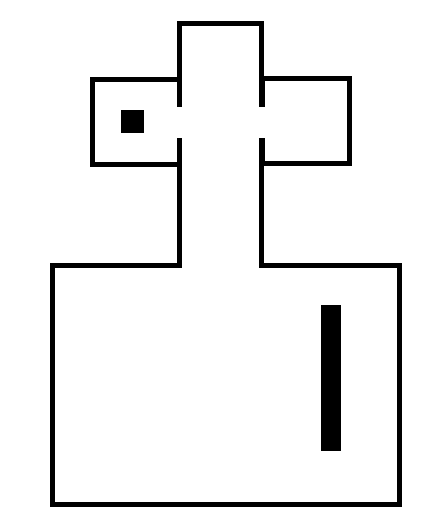
\includegraphics[width=0.5\textwidth]{figures/environment_example.png} 
\caption{Environment Design}
\label{Picture 2}
\end{figure}

\subsubsection{Mapping and Swarm Size}
For mapping I will use a occupancy grid, and the occupancy will be acquired by the E-Puck's laser sensors. 
I will yet have to decide on a resolution, for the grid.\\
I will use a swarm of 5 E-Puck robots, of which 1 will remain stationary and only function as the "Uplink point" to which all robot send the acquired data. 
The stationary robot will also be used as reference point for the localisation method.

\subsubsection{Deployment}
I am of this moment still undecided for which deployment strategy will be implemented. \\
There are 2 deployment strategies which I decided for based on the background research I have done.\\[3ex]

One of them is based on a nearest neighbour approach in which the robots will emit signals to each other which will cause them to drive away from each other until a previous maximum communication distance has been reached. This relationship between robots could be described similar to magnets which can repulse and pull in each other in order to hold a given maximum distance and thereby cover the largest possible area\\
The movement of the robots would be a random walk with included obstacle avoidance. One possibility could be to add a wall following functionality to it as well. However this would require some form of higher functions which to keep the robot from being stuck inside a loop. These higher functions could work by keeping track of the robots position on the map and react once the robot starts traversing the same area again, in this case the algorithm could force to robot back into a random walk.\\[3ex]

The other deployment strategy would implement a more controlled movement pattern. This pattern would move the robots inside a rectangular pattern which would implement a function to move around obstacles on the way before moving back into the original pattern. 
While this reason is more controlled I am not sure which one will turn out to be more effective, that it why I will implement both inside a testing phase and will then decide which of them I will use.

\begin{figure}[h]
\centering
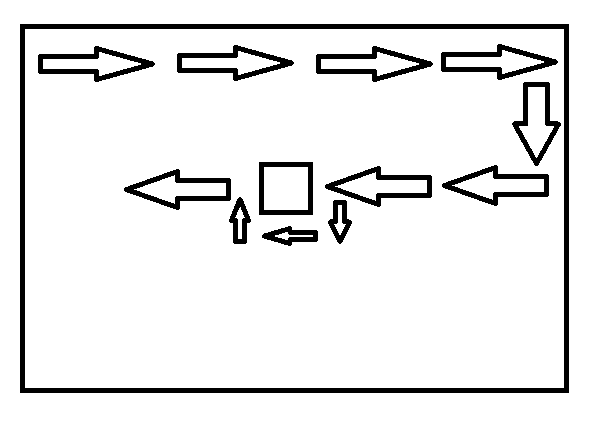
\includegraphics[width=0.5\textwidth]{figures/scanline_example.png} 
\caption{Movement pattern example}
\label{Picture 2}
\end{figure}

\section{Early Development}
After the first weeks where background reading were done and designing a plan for the final program, I started working with the Webots\textsuperscript{\texttrademark} simulator. 
\nocite{*}
\newpage
\bibliography{stk4_major_project}
\end{flushleft}
\end{document}

